\section{Statistics}

\subsection{Correlation}
Assume an inner product space.

\subsection{Linear regression}

Assume that reality can me modelled by a model like this one: 

$$ \vec{y} = \mtrx{X} \vec{w} + \vec{e} $$

Not knowing $\vec{e}$, our best guess at the outcome would be 

$$ \vec{\hat{y}} = \mtrx{X} \vec{w} $$

We can find the gradient of w by:

$$ \partDiff{E}{\vec{w}} = -  (\vec{y} - \vec{\hat{y}}) \mtrx{X}  $$



\subsection{Spatial modelling}

\subsubsection{Generalized least squares}
like linear regression, but errors are not iid, but allowed to be correlated.

\subsubsection{Gaussian processes}
Gaussian processes are a means of interpolating a value $y_x$ from surrounding values $y_x = \sum \alpha_i y_i$. Basic intuition from \href{https://bookdown.org/rbg/surrogates/chap5.html}{here}.
That is different from what linear regression or its extension GLS do: regression predicts $y$ from explanatory variables $x$, assuming a (linear) model.
Gaussian processes don't do that. They only interpolate between already observed $y$'s. No model is assumed.

Millions of surfaces $Y$ may be sampled from $N(0, \Sigma) = P(Y)$.
We call $P(Y)$ the prior. $\Sigma$ can be very large, so we assume that it can be modeled by a covariance-function $cov(h)$ which is \emph{only dependent on the distance between two points, not on the points themselves}.

\begin{lstlisting}[language=python]
import numpy as np
import matplotlib.pyplot as plt
from scipy.stats import multivariate_normal

def size(x):
    return np.sqrt(np.sum(np.power(x, 2)))

def distance(x0, x1):
    return size(x0 - x1)

def getDistanceMatrix(rowPoints, colPoints):
    rows = len(rowPoints)
    cols = len(colPoints)
    distances = np.zeros((rows, cols))
    for i in range(rows):
        for j in range(cols):
            p0 = rowPoints[i]
            p1 = colPoints[j]
            distances[i, j] = distance(p0, p1)
    return distances

def covFunction(h):
    return np.exp(- np.power(h, 2))

deltaX = 0.1
deltaY = 0.1
gridX = 20
gridY = 20
nrPoints = gridX * gridY
points = np.zeros((nrPoints, 2))
for x in range(gridX):
    for y in range(gridY):
        i = x * gridX + y
        points[i] = [x * deltaX, y * deltaY]
distances = getDistanceMatrix(points, points)

mean = np.zeros((nrPoints))
Sigma = covFunction(distances)
prior = multivariate_normal(mean, Sigma, allow_singular=True)

sample1 = prior.rvs()
sample2 = prior.rvs()
sample3 = prior.rvs()
\end{lstlisting}

\begin{figure}
    \caption{3 samples from prior $P(Y)$}
    \centering
    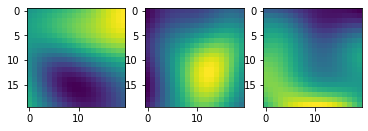
\includegraphics[width=0.7\linewidth]{images/gp_prior_samples.png}
\end{figure}

We have observed some samples $D = {(x_i, y_i)}$.
Which of these millions of surfaces are most likely given those observations? We can answer that with $P(Y|D)$.
\begin{figure}
    \caption{Observations $D$. Which field $Y$ is most likely to have produced these observations?}
    \centering
    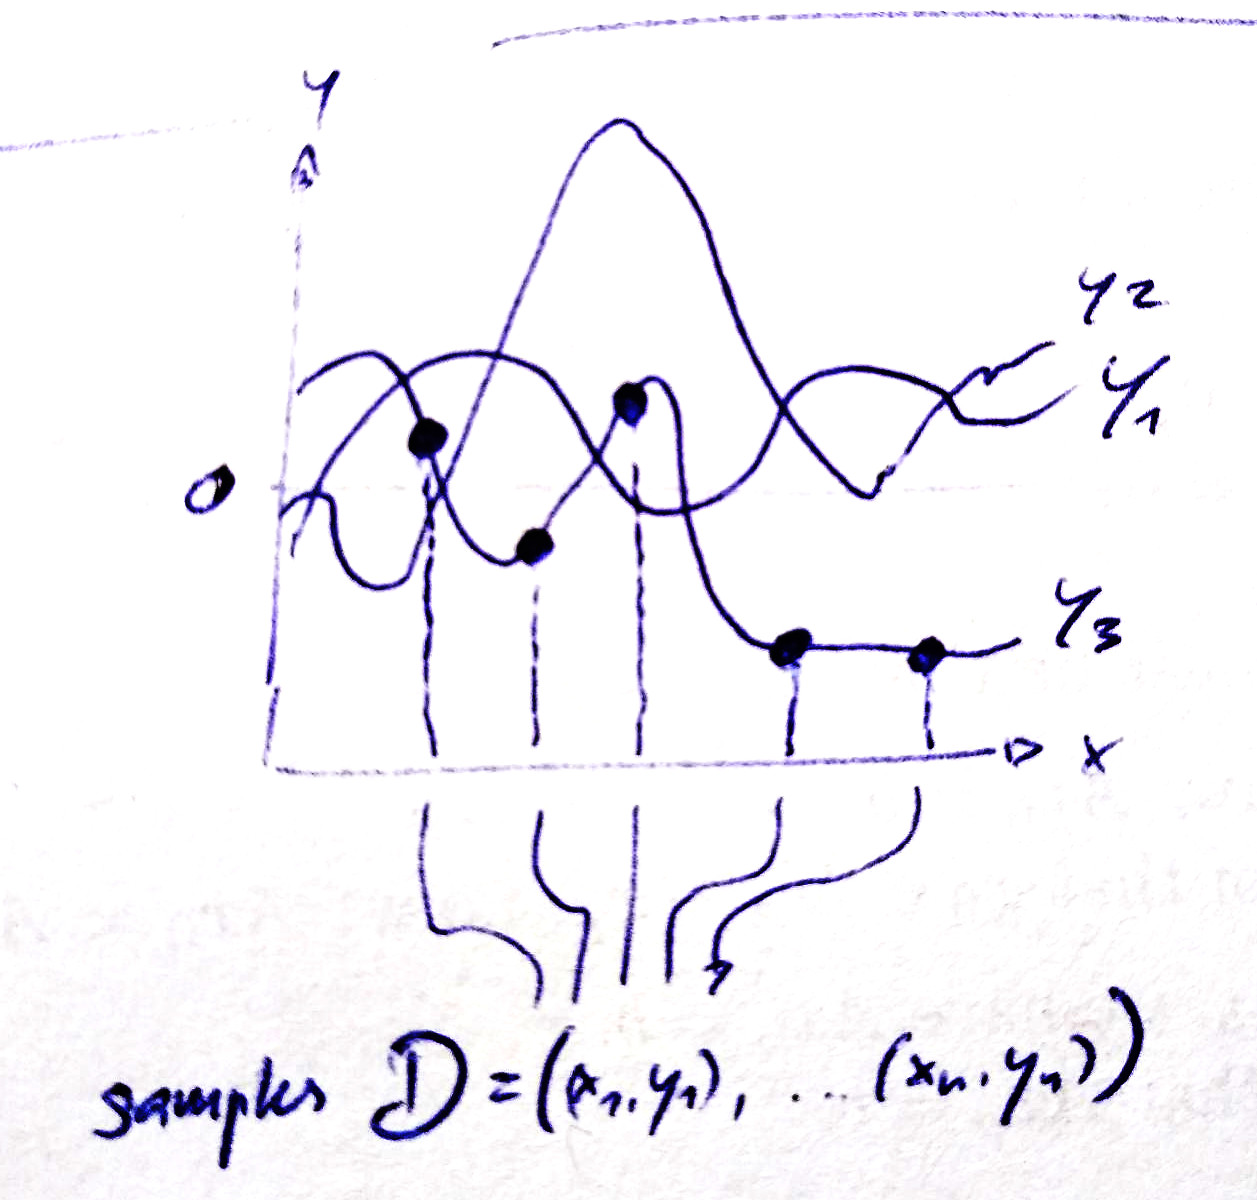
\includegraphics[width=0.4\linewidth]{images/gp_observations.jpg}
\end{figure}

We can calculate the posterior using 
$$
P(Y|D) ~ P(D|Y) P(Y)
$$
But since in gaussian processes we assume multivariate-normals, this can be done much easier.

Consider a multivariate normal distribution on, say, 400 dimensions $N(\mu, \Sigma)$. Those 400 dimensions could, for example, be pixel-values in a 20 by 20 image.
Now assume that out of those 400 dimensions we have measurements for $s$ samples, leaving a rest $r = 400 - s$.
For multivariate-normal distributions, we can easily and analytically obtain the conditional distribution $P(y_r | y_s) = N(\hat{\mu}, \hat{\Sigma})$.

Split $y$ like so:
$$ y = \myarray{y_r \\ y_s} $$
Analogously we can split the covariance-matrix:
$$ \Sigma = \begin{bmatrix}
    \Sigma_{rr} & \Sigma_{rs} \\
    \Sigma_{sr} & \Sigma_{ss} \\
\end{bmatrix}  $$

Then, according to \href{https://en.wikipedia.org/wiki/Multivariate_normal_distribution#Conditional_distributions}{wikipedia}, we can obtain $\hat{\mu}$ and $\hat{\Sigma}$ like so:
$$ \hat{\mu}_r = \mu_r + \Sigma_{rs} \Sigma_{ss}^{-1} (y_s - \mu_s) $$
$$ \hat{\Sigma}_r = \Sigma_{rr} - \Sigma_{rs} \Sigma_{ss}^{-1} \Sigma_{sr} $$

\begin{lstlisting}[language=python]
sampleIndices = np.asarray(list(map(lambda x: int(x), samples[:, 0])))
nonSampleIndices = np.asarray(list(filter(lambda v: v not in sampleIndices, np.arange(nrPoints))))
samplePoints = points[sampleIndices]
nonSamplePoints = points[nonSampleIndices]
sampleValues = samples[:, 3]

# For simplicity, we just re-calculate SigmaXX here.
# But we could have also picked the right values from Sigma
# without any need for re-computation.
distancesRR = getDistanceMatrix(nonSamplePoints, nonSamplePoints)
SigmaRR = covFunction(distancesRR)

distancesSS = getDistanceMatrix(samplePoints, samplePoints)
SigmaSS = covFunction(distancesSS)
SigmaSSInverse = np.linalg.inv(SigmaSS)

distancesRS = getDistanceMatrix(nonSamplePoints, samplePoints)
SigmaRS = covFunction(distancesRS)
SigmaSR = SigmaRS.transpose()

meanPosterior = np.matmul(np.matmul(SigmaRS, SigmaSSInverse), sampleValues)
SigmaPosterior = SigmaRR - np.matmul(np.matmul(SigmaRS, SigmaSSInverse), SigmaSR)

posterior = multivariate_normal(meanPosterior, SigmaPosterior, allow_singular=True)    
\end{lstlisting}





For more, see this \href{https://michaeloneill.github.io/GPR-tutorial.html}{very thorough tutorial}.

\subsubsection{AR and SAR}
Autoregressive and spatial-autoregressive models.

\subsubsection{Comparison}

\begin{table}[H]
    \centering
    \resizebox{\textwidth}{!}{%
    \begin{tabular}{@{}llll@{}}
    \toprule
     &
      Generalized least squares &
      Gaussian processes &
      AR \\ \midrule
    \multicolumn{1}{|l|}{type} &
      \multicolumn{1}{l|}{\begin{tabular}[c]{@{}l@{}}Predict y from x.\\ Has explanatory variables.\end{tabular}} &
      \multicolumn{1}{l|}{\begin{tabular}[c]{@{}l@{}}Interpolate y from other y's.\\ Explanatories can be added with GLS\end{tabular}} &
      \multicolumn{1}{l|}{interpolate y from other y's} \\ \midrule
    \multicolumn{1}{|l|}{model} &
      \multicolumn{1}{l|}{\begin{tabular}[c]{@{}l@{}}$y = X\alpha + \epsilon$\\ \\ $\epsilon ~ N(0, \Sigma)$\end{tabular}} &
      \multicolumn{1}{l|}{\begin{tabular}[c]{@{}l@{}}$Y ~ N(0, \Sigma)$\\ $P(Y|D) = N(\hat{\mu}, \hat{\Sigma})$\\ $\tilde{y} = \sum \alpha_i y_i$\\ Y is a field of size n by m\\ D is the observations \end{tabular}} &
      \multicolumn{1}{l|}{\begin{tabular}[c]{@{}l@{}}$y_t = \sum \alpha_i y_{t-i} + \epsilon$\\ $\epsilon ~ N(0, \sigma)$, iid \end{tabular}} \\ \midrule
    \multicolumn{1}{|l|}{Specialities} &
      \multicolumn{1}{l|}{} &
      \multicolumn{1}{l|}{\begin{tabular}[c]{@{}l@{}}$\Sigma$ is encoded using a covariance-function cov(h)\\ to save on parameters\end{tabular}} &
      \multicolumn{1}{l|}{} \\ \midrule
    \multicolumn{1}{|l|}{$\epsilon$} &
      \multicolumn{1}{l|}{} &
      \multicolumn{1}{l|}{} &
      \multicolumn{1}{l|}{} \\ \midrule
    \multicolumn{1}{|l|}{$cov(\epsilon_i, \epsilon_j)$} &
      \multicolumn{1}{l|}{} &
      \multicolumn{1}{l|}{} &
      \multicolumn{1}{l|}{} \\ \midrule
    \multicolumn{1}{l|}{$cov(y_i, y_j)$} &
      \multicolumn{1}{l|}{} &
      \multicolumn{1}{l|}{} &
      \multicolumn{1}{l|}{} \\ \bottomrule
    \end{tabular}%
    }
    \end{table}







\subsection{Tests}
Often, statistical tests work \emph{the wrong way round}. You have your hypothesis, like "these groups are different". Then you state the opposite, the \emph{null-hypothesis}. Then you determine how likely your data is under the null-hypothesis - the \emph{p-value}. And than you hope that the p-value is very low.

\paragraph{Students T-Test} compares two averages (means) and tells you if they are different from each other. The null hypothesis is that all samples come from the same distribution. That means that under $H_0$, the two means you obtained should be similar. So the interpretation goes like this: 
\begin{itemize}
    \item low p-value: the chance that your result would have happend under $H_0$ is low. It is very unlikely that the two means you have obtained actually come from the same distribution. 
    \item high p-value: It is quite possible that both your groups come from the same distribution. 
\end{itemize}
Note that there are two experimental setups that can use t-tests:
\begin{itemize}
    \item unpaired: you have two groups, with no person in both groups. Example: Test one group with medication and another with placebo. 
    \item paired: every person is first in the first and then in the second group. Example: test patients before and after treatment. 
\end{itemize}
